\documentclass{tufte-handout}

\title{GGSB 2015 Prelim} %\thanks{Inspired by Edward~R. Tufte!}}

\author[The Tufte-LaTeX Developers]{Charles Czysz}

\date{September 2015} % without \date command, current date is supplied

\setcounter{tocdepth}{3}

\geometry{bottom=0.5in}%showframe % display margins for debugging page layout

\usepackage{hyperref}
\hypersetup{
  colorlinks   = true,    % Colours links instead of ugly boxes
  urlcolor     = blue,    % Colour for external hyperlinks
  linkcolor    = black,    % Colour of internal links
  citecolor    = red      % Colour of citations
}
\usepackage{graphicx} % allow embedded images
  %\setkeys{Gin}{width=\linewidth,totalheight=\textheight,keepaspectratio}
  \graphicspath{{./figs}} % set of paths to search for images
\usepackage{amsmath}  % extended mathematics
%\usepackage{float}
\usepackage{booktabs} % book-quality tables
\usepackage{units}    % non-stacked fractions and better unit spacing
\usepackage{multicol} % multiple column layout facilities
\usepackage{lipsum}   % filler text
\usepackage{fancyvrb} % extended verbatim environments
\usepackage{amsthm}
  \fvset{fontsize=\normalsize}% default font size for fancy-verbatim environments

% Standardize command font styles and environments
\newcommand{\doccmd}[1]{\texttt{\textbackslash#1}}% command name -- adds backslash automatically
\newcommand{\docopt}[1]{\ensuremath{\langle}\textrm{\textit{#1}}\ensuremath{\rangle}}% optional command argument
\newcommand{\docarg}[1]{\textrm{\textit{#1}}}% (required) command argument
\newcommand{\docenv}[1]{\textsf{#1}}% environment name
\newcommand{\docpkg}[1]{\texttt{#1}}% package name
\newcommand{\doccls}[1]{\texttt{#1}}% document class name
\newcommand{\docclsopt}[1]{\texttt{#1}}% document class option name
\newenvironment{docspec}{\begin{quote}\noindent}{\end{quote}}% command specification environment

\newtheoremstyle{noparens}%
{}{}%
{\itshape}{}%
{\bfseries}{ - }%
{ }%
{\thmname{#1}\thmnumber{ #2}\thmnote{ #3}}

\theoremstyle{noparens}
\newtheorem*{define}{Definition}
\newtheorem*{example}{Example}

% Normal font formatting for subsections (i.e. questions)
\titleformat{\subsection}
{\large\bfseries}{\thesection}{1em}{}
%\normalfont
\usepackage{makeidx}
\makeindex


\begin{document}

\maketitle% this prints the handout title, author, and date

\noindent
\textbf{Required}

1-8: General Genetic Principles

9-12: Mapping

39-50: Study Design and Statistical Data Analysis

\vspace*{1\baselineskip}

\noindent
\textbf{Choice between}

\textbf{13-17: Genetic Architecture of Human Phenotypes}

\noindent
\textbf{or}

18-28: Population and Evolutionary Genetics

\vspace*{1\baselineskip}

29-32: Molecular Mechanisms and Model Organisms in Human Genetics

\noindent
\textbf{or}

\textbf{33-38: Gene Regulation and Human Phenotypes}

\vspace*{4\baselineskip}
\begin{abstract}
\noindent
A good answer would show in escalating order: 
\begin{itemize}
\item Basic understanding via descriptions and definition of basic terms and concepts 
\item Knowledge of biology/literature via empirical examples of concepts in action, 
\item Engagement of critical thinking by highlighting well-known limitations or novel critiques of a concept or its common application 
\item Recognition of open problems and novel research opportunities.
\end{itemize}

\end{abstract}

\newpage

\tableofcontents 

\newpage
%\printclassoptions
 
\section{General Genetic Principles}\label{sec:gen-genetic}

\subsection{1. Explain the distinction between allelic heterogeneity, genetic (locus) heterogeneity, and clinical heterogeneity. Give examples of each.}  
%\label{subsec:01}

\begin{abstract}
Great review of this topic:

\href{http://www.sciencedirect.com/science/article/pii/S009286741000320X}{Genetic Heterogeneity in Human Diseases}
\end{abstract}
%This question asks to explain how similar or identical phenotypes can have different underlying causes.

\noindent
\textbf{Overview}

\noindent
Each of the following topics have implications in the type of studies which can or cannot be used. Overall, heterogeneity ensures that large-scale association tests or case-control studies will be poorly powered to detect causal variants or genes. See the review linked above for more detail.

%\define[Allelic heterogeneity]
\begin{define}[Allelic Heterogeneity]
In a given population, different mutations in the same gene result in a similar phenotype.
\end{define}
\noindent
\textbf{Example} 

Cystic Fibrosis is caused by defective cystic fibrosis transmembrane conductance regulator proteins (CFTR). Many mutations in the CFTR gene can give rise to non-functioning proteins, which all lead to the same CF phenotype.

Two-thirds of all CF mutations are a 3bp deletion at position 508, resulting in a loss of phenylalanine. 1,500 other mutations also exist which lead to CF. However, this disease is haplosufficient..

Unknown alleleic heterogeneity can affect GWA results\footnote{\url{http://hmg.oxfordjournals.org/content/11/20/2417.short}} when LD methods are used.

\textbf{Sources}

\url{http://hmg.oxfordjournals.org/content/20/20/4082.short}

\begin{define}[Genetic (locus) heterogeneity]
Mutations in different genes result in a similar phenotype.
\end{define}

\begin{example}
The BRCA1 and BRCA2 genes are a good example of how mutations in different genes lead to the same phenotype. 
\end{example}

\begin{define}[Clinical Heterogeneity]
Variability in clinical manifestations, or phenotypes, with the same underlying mutation/genetic disorder.
\end{define}

Mutations in several genes can lead to familial hypercholesterolemia, high level of LDL cholesterol. Mutations in LDLR (LDL receptor), Apolipoprotein B, proprotein convertase subtilisin/kexin type 9 (PCSK9), and the ARH/LDLRAP1 genes can all lead to familial hypercholesterolemia.

\newpage
\subsection{2. What is the relationship between the inbreeding coefficient, kinship coefficient, and coefficient of relatedness? How are they calculated in pedigrees? Can they be estimated in the absence of pedigree information?}
\label{subsec:02} 

\begin{define}[Identity By Descent (IBD)]
Two alleles at the same locus that are descended from the same ancestral allele within the recent past. Can be 0, 1, or 2 depending on how many ancestral alleles shared between individuals.
\end{define}

\begin{marginfigure}%
  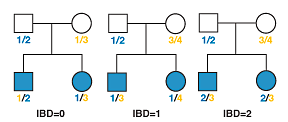
\includegraphics[scale=0.65]{./figs/ibd}
  \caption{IBD Pedigree Example}
  \label{fig:marginfig}
\end{marginfigure}

\begin{define}[Coefficient of Kinship]
$f_{xy}$: The probability that two alleles, one from person X and the other from person Y, are IBD.
\end{define}

\begin{figure}[h]
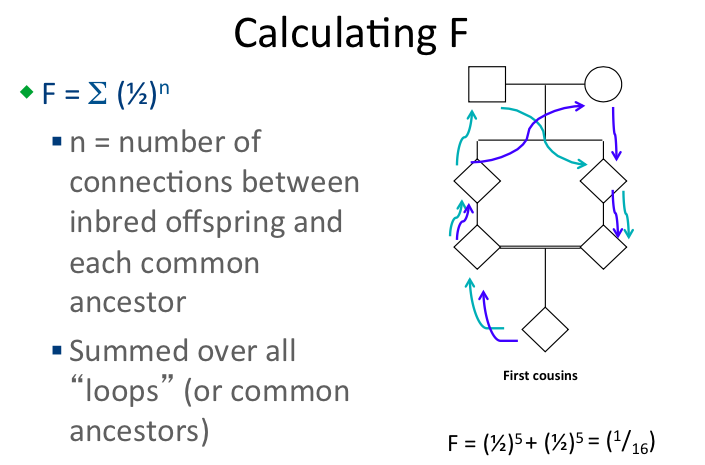
\includegraphics[scale=0.5]{./figs/kincoeff}
\end{figure}

\begin{define}[Coefficient of Relatedness]
$R_n$, the probability of sharing $n \in \{0,1,2\}$ IBD alleles. Mean relatedness, $\bar{r} = 0 \times r_0 + 1 \times r_1 + 2 \times r_2$.
\end{define}

\noindent
\textbf{Relationship between Coefficients}
\[f_{xy} = \frac{1}{2}\bar{r}\]
\begin{figure}[H]
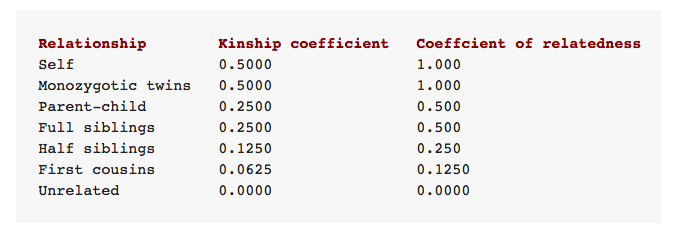
\includegraphics[scale=0.5]{./figs/kinrelate}
\caption{Relationship between Kinship and Relatedness coefficients}
\end{figure}

\begin{define}[Inbreeding Coefficient]
	$F_I$: The probability that two alleles of an individual are IBD. Since each allele is inherited from each parent, the inbreeding coefficient is equal to the coefficient of kinship for the parents. 
\end{define}

The inbreeding coefficient can capture deviations from HWE due to matings between relatives.

\begin{tabular}{c|ccc}
Genotype	& $A_1A_1$ & $A_1A_2$ & $A_2A_2$ \\ 
\hline Frequency	& $p^2(1-F_I) + pF_I$ & $2pq(1-F_I)$ & $q^2(1-F_1) + qF_I$ \\ 
Fitness	& 1 & $1-hs$ & $1-s$ \\ 
\end{tabular} 

\noindent
\textbf{Estimation without Pedigrees}

Genotype data can be used to estimate the inbreeding coefficient between individuals using computational tools such as PLINK.

\newpage
\subsection{3. What are the key distinguishing characteristics of pedigrees segregating autosomal dominant, autosomal recessive, X-linked, Y-linked, and mitochondrial diseases?}
\label{subsec:03}

 \noindent
 \textbf{Autosomal Dominant}
 
 Both sexes are equally affected. Offspring have a 50\% chance of inheriting the disease from an affected parent.
 
 \noindent
 \textbf{Autosomal Recessive}
 
 If both parents are carriers, then $\frac{1}{4}$th of offspring will show a disease phenotype. May appear to skip generations residing in a heterozygous carrier state instead of homozygous affected.
 
 \noindent
 \textbf{X-linked Dominant}
 
Affected men always pass disease to daughters. Affected women have $\frac{1}{2}$ths chance of passing disease to offspring.
 
 \noindent
 \textbf{X-linked Recessive}
 
Women can be either affected or carriers. Men always affected. Colorblindness as an example.
 
\noindent
\textbf{Y-linked}

Affected fathers always pass to sons, never to daughters.

\noindent
\textbf{Mitochondrial}

Passed on only by mothers to all offspring.
 
\newpage
\subsection{4. Explain the "non-Mendelian" concepts of uniparental disomy and imprinting. How would these be manifested in pedigrees and how are they demonstrated at the cellular or molecular levels?}
\label{subsec:04}

\begin{define}[Mendelian Genetics]
Involves the "Laws" of random segregation, independent assortment, and dominance. Non-Mendelian genetics violate at least one of these assumptions.
\end{define}

\begin{define}[Uniparental Disomy]
Offspring inherits a chromosome, or part of one chromosome, from one parent only. These offspring are euploid, but with an unequal contribution of genetic material from the parents.
\end{define}

Uniparental disomy can manifest in two ways: inheriting both homologs from one parent (heterodisomy), or duplication of a single inherited chromosome (isodisomy).

\textbf{Heterodisomy}

Offspring inherits homologs from one parent only. Can occur during a nondisjunction error in Meiosis I, where one daughter cell inherits both sister chromatids while the other inherits none. This will lead to trisomy after fertilization, and heterodisomy if trisomy rescue occurs and results in the loss of the allele from the other parent.

Heterodisomy can also result from crossover events. In the parental generation, a cross between a balanced translocation carrier and a normal carrier can result in partial heterodisomy if the offspring inherits a crossover product and non-crossover product. However, this is an unbalanced gene load and is less prone to survival (10-15\% incidence versus theoretical 50\%).

In a Robertsonian translocation, acrocentric chromosomes fuse to create a single fusion chromosome. If this translocation occurs between homologs and is passed down to offspring, trisomy occurs (eg Trisomy 21). If, however, the non-fusion chromosome is lost by trisomy rescue, then heterodisomy occurs.

In a pedigree analysis, heterodisomies result in a parent passing their recessive condition to an offspring. Additionally, the parents of the affected parent are carriers. 

\textbf{Isodisomy}

Isodisomy occurs when a single parental homolog is inherited and duplicated. This can occur after nondisjunction events in both Meiosis I and II. While the Meiosis I error gives 2 gametes which can result in heterodisomy, the other two gametes result in isodisomy if chromosomal duplication occurs. In this case, the other parental chromosome is duplicated.

During a meiosis II error, the sister chromatids fail to separate, leaving one product with two copies of the same chromosome in one gamete and none in the other. For the former gamete, trisomy rescue and loss of the other parent's chromosome leads to isodisomy. For the latter gamete, duplication of the other parental chromosome leads to isodisomy.

In a pedigree analysis, isodisomy should be suspected when an offspring shows a recessive disease when only one parent is a carrier. This suggests that the recessive allele was inherited and duplicated.
 
 \textbf{Discovering Uniparental Disomy}
 
 Discrepancies between karyotypes of placenta and fetus.
 
 Mosaicism of normal and trisomic cells (rescue occurs after first cell division).
 
 Abnormal chromosome structure giving evidence of inheritance of Robertsonian product or unbalanced products. Usually seen by FISH.
 
 Other DNA tests:
 
 Test for STR (short tandem repeats) of known high heterozygosity, genotyping parents and offspring. 

\begin{define}[Imprinting]
Imprinting results from the inheritance of epigenetic marks silencing an allele in a parent-of-origin specific manner.
\end{define}

With imprinting, only one allele is expressed, and which allele depends on its parent-of-origin. When uniparental disomy of an imprinted allele occurs, the resulting expression can either go to 0x or 2x depending on if the silenced allele is the one doubled or not.

 \textbf{Sources}
 
 \url{http://www.nature.com/gim/journal/v3/n3/full/gim200144a.html}
 
\newpage
\subsection{5. What evidence is there for the presence of modifier loci? How is this related to the concept of epistasis and how is it distinct (or not) from polygenic and other models of inheritance?}
\label{subsec:05}

\begin{define}[Modifier loci]
A loci or gene which alters the expression of another gene, usually through epistatic interactions.
\end{define}

Modifier loci usually considered part of the genetic background. Thus, some modifier loci can have no effect on wildtype phenotypes but can affect mutant phenotypes.

In epistatic interactions, modifier loci do not lead to binary traits (present or absent, etc), but result in a gradient of phenotypes (coat color in dogs and horses). Can enhance, suppress, normalize, and enhance pleiotropy. These modifier loci usually act on or within the same biological pathway as the gene they affect.

\noindent
\textbf{Evidence}

Clinical variability in disease manifestation despite identical genotypes at the risk loci. Many exist in mice, but fewer found in humans due to difficulty to study.

Variation in phenotype without variation in genotype. 

\noindent
\textbf{Mode of Inheritance}

The inheritance of modifier loci cannot be accurately described by Mendelian or polygenetic modes of inheritance. Modifier alleles not strictly dominant or recessive, but depend on other alleles. For example, a dominant negative modifier loci only destroys a phenotype when inherited with a mutant allele in the same pathway.

In the polygenic model of inheritance, alleles affecting a phenotype act independently and with small, additive effect sizes. Thus only the total allele count matters. With modifier loci, the presence or absence of a particular allele determines the phenotype. Not only do alleles affecting a phenotype matter, but alleles affecting those alleles do also.

\newpage
\subsection{6. What are distinctions among the concepts linkage, linkage disequilibrium, and association? Under what circumstances would each be preferable for genetic mapping? Consider both sample composition and types of diseases.}
\label{subsec:06}

\begin{define}[Linkage]
Two loci which tend to be inherited together due to low probability of recombination.
\end{define}

Using data from many recombinations, linkage maps were created to map loci relative to the proportion of recombinations between them. In units of map units \textbf{m.u.} or centiMorgans. 1 mu is defined as the distance between genes with 1/100 meiosis products as recombinant. 

\noindent
\textbf{Parametric Linkage Mapping}

Useful when samples are from large and informative pedigrees. Informative indicates that each allele can be assigned to 	a specific parent.

Calculate LOD scores by finding the MLE of $\theta$

\[ \text{LOD} = \log \frac{(1-\theta)^{NR}\theta^R}{0.5^{NR+R}} \]

\noindent
\textbf{Nonparametric Linkage Mapping}

Used when the underlying model is unknown. Use affected relatives in order to leverage degree of allele-sharing. Estimate IBD between affected relatives. Look for alleles shared between affected individuals more often than chance.

\noindent
\textbf{Linkage mapping usefulness}

Linkage mapping is useful with large and informative pedigrees. Mapping also requires easily genotyped markers providing good resolution of genome cover. Linkage mapping also best identifies Mendelian genes with high penetrance.

\begin{define}[Linkage Disequilibrium (LD)]
Non-random association of alleles at multiple loci.
\end{define}

LD is measured using a variety of statistics, the most common is the difference between expected heterozygosity and observed heterozygosity.

LD decreases each generation due to recombination. Including LD information in linkage analyses can increase power. 

\textbf{Limitations}

LD models assume constant population size and drift-recombination equilibrium. Population structure can artificially inflate LD estimates.

\begin{define}[Association Studies]
Utilizing a large sample of unrelated cases and controls to determine which, if any, tag SNPs are more associated with a disease than not.
\end{define}

The most common, now, association study is GWAS. In GWAS, measure associations with common (MAF > 5\%) SNPs and a phenotype of interest. Using a large cohort of people in the same population increases power to detect associations.

\newpage
\subsection{7. Define epistasis. Describe approaches that allow epistasis to be detected or quantified. Describe some biological mechanisms that can produce epistasis. Discuss the implications of epistasis for efforts to map the genetic causes of phenotypes. Discuss the potential implications of epistasis for the evolutionary process.}
\label{subsec:07}

Multiple types of epistasis observed:

\begin{itemize}
\item \textbf{Functional} - Genes in the same pathway
\item \textbf{Compositional} - 
\item \textbf{Statistical}
\end{itemize}

\noindent
\textbf{Effect of epistasis on mapping}

An epistatic interaction might prevent identifying an association with one loci and a phenotype depending on 
\newpage
\subsection{8. Define heritability. Describe methods used to quantify the heritability of a phenotype. Discuss the value and limitations of heritability as a descriptor of the extent to which a phenotype has genetic causes. Describe the "missing heritability problem" and its potential explanations.}
\label{subsec:08}

A measurable phenotypic trait varies within a population. Beak length in finches is a good example: there exists a mean length, but the values can be higher or lower. This variance is denoted by $\sigma_P^2$.

For most traits, the phenotype is made up of contributions from genes and environment, and similarly for the variance.

\[ \sigma_P^2 = \sigma_G^2 + \sigma_E^2 \]

The relationship between genetic variability and phenotypic variability is deemed heritability. 

\[ h^2 = \frac{\sigma_a^2}{\sigma_P^2} \]

Where $\sigma_a^2$ is the additive genetic variance (as opposed to dominance effects).

An estimate of $h^2$ can be found by plotting the phenotypic value of offspring versus the midparent value and fitting a linear regression. The slope of this regression estimates $h^2$, how well the parent phenotype determines the offspring phenotype.

\textbf{Twin Method}

Twin studies allow the inflation of heritability by common environment to be minimized. Since twins are presumed to have experienced the same environment growing up, the environmental variance is the same. Comparing monozygotic twins to dizygotic twins will allow a better estimation of heritability. 

\textbf{Considerations}

Calculations of heritability can be influenced by shared environment. Thus, heritability is usually specific to a single population or region.

\textbf{GCTA}

\textbf{Missing heritability}

A heritability of 1 indicates that a genetic variant or variants can explain all of the phenotypic variance. As association studies and GWA studies have increased sample size and tagged variants, the heritability measures of measured traits has not increased as quickly.

\newpage
\section{Mapping}\label{sec:map}

\subsection{9. What is the difference between an odds ratio and relative risk? When would you use each and how might these relate to the concept of heritability in a genetic study?}

\begin{define}[Relative Risk]
$\lambda_R$ is the risk that an affected person acquires a trait divided by the risk for the general population.
\end{define}

Consider a 2x2 contingency table testing a response (yes or no) based on group (placebo versus medicine). $\pi_1$ is defined as the probability of a "yes" response for the placebo group. $\pi_2$ is the probability of a "yes" response for the medicine group.

\begin{table}
\centering
\begin{tabular}{llll}
\toprule
Group & Diseased & Not Diseased & Total\\
\midrule
Placebo & $\pi_1$ & $1-\pi_1$ & 1\\
Medicine & $\pi_2$ & $1-\pi_2$ & 1\\
\bottomrule
\end{tabular}
\end{table}

The relative risk for this table is given by \[ \text{relative risk} = \frac{\pi_1}{\pi_2} \]

Example Data:

\begin{table}
\centering
\begin{tabular}{llll}
\toprule
Group & Diseased & Not Diseased & Total\\
\midrule
Placebo & 189 & 10,845 & 11,034\\
Medicine & 104 & 10,933 & 11,037\\
\bottomrule
\end{tabular}
\caption{Adapted from Table 2.3 from \emph{Introduction to Categorical Data Analysis} by Alan Agresti}
\end{table}

In this example, $\hat{\pi_1} = \frac{189}{11,034}$ and $\hat{\pi_2} = \frac{104}{11,037}$. A small difference, but a relative risk of 1.83, meaning the placebo group is 83\% more at risk than the medicine group.

\begin{define}[Odds]
Expected ratio of successes. Define $p$ as probability of success, $\text{odds}_1 = \frac{p}{1-p}$. Thus, an odds of 3 indicates a probability of success of 0.75 and of failure 0.25.
\end{define}

For the previous table, we can define the odds ratios for each group, giving $\text{odds}_1 = \frac{\pi_1}{1-\pi_1}$ and $\text{odds}_2 = \frac{\pi_2}{1-\pi_2}$, respectively. 

\begin{define}[Odds Ratio]
A ratio of odds. For a 2x2 contingency table, $OR = \theta = \frac{\text{odds}_1}{\text{odds}_2}$.
\end{define}

Odds ratios of 1 describe the null hypothesis that the group and response are independent. When $\theta > 1$, the odds of success for group 1 are $\theta$ times higher than for group 2. When $\theta < 1$, the odds of success for group 2 are $\frac{1}{\theta}$ times higher than for group 1.

\begin{define}[Log Odds]
As a fraction of positive values, the odds ratio is only lower-bounded by 0. Thus, the distribution is very skewed. Taking the log odds removes this skewedness since it is symmetric around its null value of 0.
\end{define}

\textbf{Relative Risk versus Odds Ratio}

Recall that \[ \text{RR} = \frac{\pi_1}{\pi_2} \] and \[ \text{OR} = \frac{\pi_1 / (1-\pi_1)}{\pi_2 / (1-\pi_2)} \]

Thus, \[ OR = RR \times \frac{1-\pi_2}{1-\pi_1} \] and when the probabilities of success are both small, the RR and the OR are very similar.
 
 \noindent
 \textbf{Odds Ratio and Heritability}
 
 In GWAS, many variants show low effect sizes with OR between 1 and 1.3. However, GWAS might miss variants with very low OR (e.g 1.05), thus contributing to the missing heritability problem. 
 
 \textbf{Sources}
 
 Lander and Schork. "Genetic Dissection of Complex Traits" 1994. \emph{Science}
 
\newpage
\subsection{10. What are the differences between quantitative and qualitative trait mapping, correlated phenotypes, multi-trait mapping?}

\textbf{Qualitative versus Quantitative Traits}

Qualitative traits are those of categorical, rather than numeric, values. Coat color in rats is one example (black, white, or brown). Quantitative traits, on the other hand, are phenotypes which can be measured along a continuous range (tail length, in centimeters), assumed to be normally distributed within a population. Qualitative trait mapping is useful for Mendelian inheritance while quantitative trait mapping is better for traits with multiple underlying causative loci.

\textbf{Trait Mapping}

Trait mapping allows the interrogation of the genetic region associated with a phenotypic trait. 

Qualitative trait mapping requires:

\begin{itemize}
\item Separate phenotypic categories
\item Many genetic markers
\item Inbred line for crosses
\end{itemize}

Quantitative trait mapping requires precise genotypes at many loci, since it measures the correlation between allele count and phenotype value.

\newpage
\subsection{11. Describe the impact of using subjects with varied degrees of relatedness in an association study. How can this be addressed?}

\noindent
\textbf{Using related individuals}

One reason to include related individuals in a study is to increase the power to detect rare variants passed down through a family. 

Related genomes can be used to correct for sequencing errors (differentiating a SNP or indel) and to allow imputation to cheaply genotype others after deeply genotyping a few.

Family-based association tests are performed using the transmission distortion test. 

\textbf{Kinship Matrix}

The relatedness between subjects is calculated in a kinship matrix, an $nxn$ matrix of correlations between genotyped markers. This matrix can be included as a covariate in a linear model to account for different relatedness between individuals.

\noindent
\textbf{Potential Impacts}

In GWA or other association studies, having a high proportion of related individuals in the sample can yield spurious results, or mask true results, due to non-random differences in allele frequency. This problem is similar to having population structure, therefore identifying and removing the effects of relatedness is similar.

\newpage
\subsection{12. What are the strategies used to identify causal variants within an LD block associated with a trait? How do you assign a target gene as connected to a non-coding variant associated with a trait? How do you prioritize variants as likely causal/ how do you experimentally test them?}

Due to LD, many variants can be shown to associate with a particular phenotype. Also due to LD, the most associated variant may not be the causal variant, but in high LD with the causal variant. This usually arises from relatively low genotyping coverage (not all variants will be typed).

\noindent
\textbf{Fine Mapping}
When a candidate region is found in GWAS, fine mapping studies are used to determine the causal variant. Fine-mapping studies rely on both a high number of genotypic markers and high recombination rates. These two factors allow precise identification of markers segregating with a phenotype of interest.

\noindent
\textbf{Connecting noncoding variants to genes}

Non-coding variation can still play a role in gene expression and activity by affecting how it is transcribed. Variation in promoters, enhancers, introns, and other regions can cause differential gene regulation, affecting a trait of interest. 

Functional genomic techniques can be used to assign variants to functional elements in the genome. If a variant overlaps or is near an element, the most likely mechanism of action for that variant is explained by the regulatory element.

\noindent
\textbf{Prioritizing variants as causal}

\emph{Functional annotations} - Overlap variants with functional elements to see any correlations with regulatory elements or other mechanisms of affecting genes

\emph{Nucleotide-level analysis} - Determine if the variant affects a motif.

\emph{Conservation} - Compare variants to related species to determine conservation. Areas under selective constraint relative to surrounding regions can be assumed biologically important

\emph{Network analysis} - 

\newpage
\section{Genetic Architecture of Human Phenotypes}\label{sec:genarch}
\subsection{13. What is "genetic architecture" in the context of diseases and traits? What methods do we have for understanding genetic architecture and how would you characterize the relative power and resolution among these tools? What practical reasons are there for having a good understanding of it? What if any value is there in knowing general features of architecture in the absence of complete and detailed knowledge?}

Genetic architecture refers to how natural genotypic features leads to phenotype. For diseases and traits, it can refer to genes, modifier loci, functional elements, etc. Additionally, the frequencies of each allele at each loci is accounted for.

Different genetic architectures underlie the differences between simple and complex diseases. The former is causes by one allele, while the latter is due to a combination of alleles.

\textbf{Methods}

\emph{Genetic Screens}

\emph{Linkage Mapping}

\emph{Association Studies}

\noindent
\textbf{Importance}

Understanding the genetic architecture of a trait/disease of interest can inform proper study design.  
\newpage
\subsection{14. What are the expected relationships between allele frequency spectrum, penetrance, and prevalence of genetic disease?}

\begin{define}[Allele frequency spectrum]
AFS is defined as the frequency of all alleles of a given gene.
\end{define}

The frequency of allele $a$ is given by \[\frac{a}{N*n} \] for a population of $N$ individuals with poloidy $n$ and $a$ copies of the $a$ allele.

\begin{define}[Prevalence]
In a population, the prevalence of a disease is the proportion of individuals affected.
\end{define}

\begin{define}[Penetrance]
For pedigrees, penetrance is the proportion of affected individuals given a particular genotype.
\end{define}

The prevalence of a disease can be estimated from its penetrance in a representative sample. Since penetrance is the proportion of affected individuals who have the risk allele, the population-wide prevalence is the product of the penetrance, population size, and allele frequency.

There is an expectation that the more penetrant an disease-causing allele is, the stronger the selection against it, and the lower the frequency it will reach in a population. This assumption works well for Mendelian diseases, but is less important for complex disease where the underlying architecture can involve many loci of small effects. 

These loci experience weak selection, making genetic drift the main driving force of allele frequency changes. 

\newpage
\subsection{15. What are the assumptions of the polygenic model of quantitative traits and of binary (disease) traits? What are alternative models?}

The polygenic model of quantitative traits assumes a polygenic phenotype is due to additive interactions of alleles at many loci. Each loci serves as a binomial random variable, and the sum of multiple loci result in a normal distribution describing the distribution of number of additive alleles in a population.

\textbf{Assumptions}

\begin{itemize}
\item Alleles have small effects on phenotype
\item Effects are additive
\item No dominance
\item No epistatic or gene by gene interactions
\item Loci are independent, i.e. no linkage
\item Environmental variance is minimal
\end{itemize}

\noindent
\textbf{Binary Traits}

Most disease phenotypes are classified as categorical variables. For example: has disease or doesn't have disease. Or any grades of disease severity. This seems different from polygenic traits which occupy a continuous range of phenotypic values.

For many binary traits, there exists an underlying \emph{liability} which is polygenic in nature. This model assumes that, at a specific phenotypic value, the disease classifier switches from not diseased to diseased. In this way, individuals with phenotype values above the threshold are diseased, while those below are not diseased.

\newpage
\subsection{16. Discuss and contrast the common versus rare allele hypotheses to explain the genetic architecture of human diseases. What are the implications of each hypothesis for mapping strategies, including association studies and large-scale sequencing efforts?}

\newpage 
\subsection{17. How noncoding variants lead to phenotypic variation? What do we know about the role of enhancers in Mendelian disease? What's the evidence for enhancer variation in complex disease? Do enhancer variants have small or large effects n disease phenotypes?}

\newpage
\section{Gene Regulation and Human Phenotypes}\label{sec:genreg}
\subsection{33. Critically review the evidence and mechanisms of transgenerational epigenetic inheritance.}

\newpage
\subsection{34. Discuss the theoretical impact of epigenetic phenomena on association studies.}

\newpage
\subsection{35. Define eQTL mapping. Discuss the insight we gained from eQTL mapping on gene regulation, on the genetic architecture of phenotypes. Discuss their utility for understanding the genetic bases of human diseases.}

eQTL mapping is a subset of QTL mapping, where the phenotype of interest is gene expression. In eQTL studies, genotype dosage is correlated with gene expression. Significant hits are loci where a change in genotype dosage is correlated with an additive change in genotype.

eQTLs can exist in \emph{cis} and \emph{trans}. \emph{cis}-eQTLs are defined by a distance cutoff to nearby genes, while \emph{trans}-eQTLs can act genome-wide. There is much more power to detect eQTLs in \emph{cis} than in \emph{trans}. Most \emph{cis}-eQTLs are located near the TSS of the target gene, and decrease in frequency as the distance from the TSS increases.

\noindent
\textbf{eQTLs and Genetic Architecture}

eQTL analyses have revealed a more complex architecture to certain diseases: not only is there a new risk lock, but the alleles at that loci act additively. Additionally, these loci exhibit high heritibility in explaining much of the variance in transcript abundance for a given gene.

\newpage
\subsection{36. Histone modifications: what we know about their role in gene regulation.}

\newpage
\subsection{37. Network motifs in biology. Examples of regulatory circuits and their function.}

\newpage
\subsection{38. Robustness and redundancy in biological functions. How do they evolve and how are they being maintained?}

\newpage
\section{Study Design and Statistical Data Analysis}\label{sec:stats}

\subsection{39. Normalization of genomic data: why it is needed and what assumptions are required.}

Standardization and normalization are important when considering data from the same biological source across different technical replicates. Technical variation can introduce unwanted noise onto an underlying biological distribution, so removing that noise is the goal.

Normalization casts data into a predefined range while standardization casts the data to have mean 0 and variance 1. Applying both yields the standard normal distribution used in Z-tests. 

Normalization is necessary for allowing comparisons of biological and technical replicates. Despite coming from the same source type, random variation can alter the distribution of the measurements without reflecting differences in biology.

\noindent
\textbf{Assumptions}

\begin{itemize}
	\item All samples share the same underlying distribution
	\item Experimental treatments affect a small number of genes
	\item Noise is additive
\end{itemize}

\newpage
\subsection{40. Accounting for confounding factors (e.g., batch effect) in genomic data: methods to test and correct for such effects.}
\begin{define}[Batch]
Variables differing between samples where the difference is not due to measured variables. Examples include sequencing machine, technician, etc.
\end{define}

Batches can introduce bias in measurements, and must be minimized in experimental design. However, if there is a batch effect in the data, identifying and correcting are important.

\noindent
\textbf{Identifying}

The easiest way to identify batches is by keeping records of all sample preparation and including them as cofactors in the linear model. Computationally, PCA and clustering methods can identify batches to include as factors. 

\newpage
\subsection{41. Effective design for genomic studies (how to replicate? how to account for confounding factors? when and how to pool samples? variance vs. bias).}

\newpage
\subsection{42. Be familiar with the use of Principal Components Analysis (and related dimension reduction techniques) in genetic applications.}

PCA is a matrix decompositon method which yields orthogonal vectors along the axes of highest variance. PCs are calculated such that the first PC represents the axis of highest variance, with subsequent PCs representing lower variances.

PCs can represent batch effects, especially with regard to population structure. If structure exists within a genetic matrix, the top PCs will capture much of the variation due to population, and points will cluster by population. 

\textbf{Caveats}

PCA is sensitive to differences in sample sizes.

Can be unclear as to what each PC represents.

Including too many in the model can remove signal instead of noise.

\newpage
\subsection{43. Be familiar with methods for identifying population structure and admixture.}

\newpage
\subsection{44. Genotype imputation: how does it work, how is it used?}

\newpage
\subsection{45. What is a Hidden Markov Model?}

\newpage
\subsection{46. Describe the principles behind statistical methods for inferring haplotypic phase from simple pedigrees (eg parent-child trios), and samples of unrelated individuals.} 

\newpage
\subsection{47. Describe how to fit a linear model and test for significance of effects. What does a p value of 0.05 (or 0.01, or any other value) mean?} 

\newpage
\subsection{48. What issues affect your assessment of whether an observed association is likely to be real?}

\newpage
\subsection{49. Describe the principles underlying the use of False Discovery Rates in Genomic studies.}

FDR is a method used to correct for multiple testings, which inflate the Type I error rate as the number of tested hypotheses increases.

In genetic tests, the likelihood of seeing a significant p-value increases as the number of tests increases (i.e. associations for 1,000,000 SNPs or 20,000 genes).

The Benjamini-Hochberg method is the most widely-used. For independent null hypotheses $H_1 ... H_m$ and corresponding p-values $P_1 ... P_m$,

\begin{itemize}
	\item For an FDR $\alpha$, find the largest $k$ s.t. $P_k \leq \frac{k}{m}\alpha$
	\item Then, reject all hypotheses $H_i$ for $i = 1,...,k$
\end{itemize}

In this way, the FDR represents the number of significant hits which are false, instead of the Type I proportion of false positives in all tests.

\begin{tabular}{c cc|c}
	  & Do not reject & Reject & Total \\ 
 $H_0$ True & U & V & $m_0$ \\ 
 $H_1$ True & T & S & $m_1$ \\ 
	\hline Total & W & R & $m$ \\  
\end{tabular} 

A p-value significance cutoff measures Type I error as V/m, while q-values set the FDR at V/R.

\textbf{Comparison with Family-wise error rate correction}

The most common FWER correction is the Bonferroni correction, defined as $\alpha* = \frac{\alpha}{m}$, where $\alpha$ is the initial p-value significance and m is the number of hypothesis tests. This cutoff is much more conservative than FDR, in that fewer tests will be found significant, inflating the Type II error rate. FDR also gives tests greater power than Bonferroni corrections.


\newpage
\subsection{50. Describe Bayes Theorem and be familiar with its application in genetics.}
\end{document}
